% Options for packages loaded elsewhere
\PassOptionsToPackage{unicode}{hyperref}
\PassOptionsToPackage{hyphens}{url}
%
\documentclass[
]{article}
\usepackage{amsmath,amssymb}
\usepackage{iftex}
\ifPDFTeX
  \usepackage[T1]{fontenc}
  \usepackage[utf8]{inputenc}
  \usepackage{textcomp} % provide euro and other symbols
\else % if luatex or xetex
  \usepackage{unicode-math} % this also loads fontspec
  \defaultfontfeatures{Scale=MatchLowercase}
  \defaultfontfeatures[\rmfamily]{Ligatures=TeX,Scale=1}
\fi
\usepackage{lmodern}
\ifPDFTeX\else
  % xetex/luatex font selection
\fi
% Use upquote if available, for straight quotes in verbatim environments
\IfFileExists{upquote.sty}{\usepackage{upquote}}{}
\IfFileExists{microtype.sty}{% use microtype if available
  \usepackage[]{microtype}
  \UseMicrotypeSet[protrusion]{basicmath} % disable protrusion for tt fonts
}{}
\makeatletter
\@ifundefined{KOMAClassName}{% if non-KOMA class
  \IfFileExists{parskip.sty}{%
    \usepackage{parskip}
  }{% else
    \setlength{\parindent}{0pt}
    \setlength{\parskip}{6pt plus 2pt minus 1pt}}
}{% if KOMA class
  \KOMAoptions{parskip=half}}
\makeatother
\usepackage{xcolor}
\usepackage[margin=1in]{geometry}
\usepackage{graphicx}
\makeatletter
\def\maxwidth{\ifdim\Gin@nat@width>\linewidth\linewidth\else\Gin@nat@width\fi}
\def\maxheight{\ifdim\Gin@nat@height>\textheight\textheight\else\Gin@nat@height\fi}
\makeatother
% Scale images if necessary, so that they will not overflow the page
% margins by default, and it is still possible to overwrite the defaults
% using explicit options in \includegraphics[width, height, ...]{}
\setkeys{Gin}{width=\maxwidth,height=\maxheight,keepaspectratio}
% Set default figure placement to htbp
\makeatletter
\def\fps@figure{htbp}
\makeatother
\setlength{\emergencystretch}{3em} % prevent overfull lines
\providecommand{\tightlist}{%
  \setlength{\itemsep}{0pt}\setlength{\parskip}{0pt}}
\setcounter{secnumdepth}{-\maxdimen} % remove section numbering
\ifLuaTeX
\usepackage[bidi=basic]{babel}
\else
\usepackage[bidi=default]{babel}
\fi
\babelprovide[main,import]{spanish}
% get rid of language-specific shorthands (see #6817):
\let\LanguageShortHands\languageshorthands
\def\languageshorthands#1{}
\ifLuaTeX
  \usepackage{selnolig}  % disable illegal ligatures
\fi
\usepackage{bookmark}
\IfFileExists{xurl.sty}{\usepackage{xurl}}{} % add URL line breaks if available
\urlstyle{same}
\hypersetup{
  pdftitle={Avance de la calificación de informes de supervisión},
  pdfauthor={Luis Palacios Sánchez (TF-II)},
  pdflang={es},
  hidelinks,
  pdfcreator={LaTeX via pandoc}}

\title{Avance de la calificación de informes de supervisión}
\author{Luis Palacios Sánchez (TF-II)}
\date{2025-04-15 16:49:41 America/Lima}

\begin{document}
\maketitle

\begin{center}\rule{0.5\linewidth}{0.5pt}\end{center}

\section{Reporte de emisión documentaria
DFAI}\label{reporte-de-emisiuxf3n-documentaria-dfai}

El presente reporte busca realizar un adecuado seguimiento al registro
en la \textbf{Herramienta de Calificación de Informes}, elaborado por la
DFAI. Esta herramienta, la cual fue lanzada el 10 de enero de 2025,
busca analizar la la calificación de forma y fondo de los informes de
supervisión, de acuerdo a lo indicado por la directora.

\subsection{Ingresos}\label{ingresos}

Al cierre de mes de marzo\footnote{1} se reportó el ingreso de
\textbf{264} informes entre enero y febrero a la DFAI, sin embargo,
entre febrero y abril se han registrado solo \textbf{212} informes en el
aplicativo. .

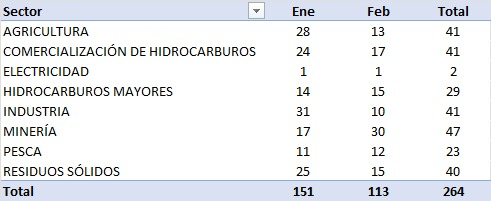
\includegraphics[width=0.8\linewidth]{../../2) INPUT/META MARZO}

\newpage

\subsection{Evolución del registro}\label{evoluciuxf3n-del-registro}

El registro Como puede observarse en el siguiente cuadro, el ritmo de
registro incrementó a lo largo de marzo, sin embargo, debe alcanzar a
cubrir el flujo de entrada de informes para cada área.

A nivel de subsector también resulta importante cubrir el flujo de
ingreso de informes

\newpage

\subsection{Brechas}\label{brechas}

Finalmente como puede observarse en ta tabla contigua, a nivel actos
administrativos pendientes de emisión se tiene el siguiente detalle:

\begin{itemize}
\tightlist
\item
  RSD: Hidrocarburos y minería son los subsectores con mayor cantidad de
  pendiente, representando el 12.1\% y 19.7 \% del total de sus
  expedientes, sin embargo, consultoras ambientales presenta el mayor
  ratio de todos.
\item
  IFI: Hidrocarburos e industria presentan la mayor cantida de IFI
  pendientes, representando el 3\% y 6.6\% de los expedientes, sin
  embargo agricultura presenta el mayor ratio con el 15.6\%.
\item
  RD: Hidrocarburos presenta la mayor cantidad de expedientes con RD
  pendientes con 59 expedientes, representando el 3.2\% de los
  expedientes, sin embargo, agricultura presenta el mayor ratio con el
  4.7\%.
\end{itemize}

Finalmente, se recomienda evaluar los datos brindado con prudencia en la
medida que este reporte se encuentra en periodo de prueba a la espera de
sus comentarios, observaciones o sugerencias.

\begin{center}\rule{0.5\linewidth}{0.5pt}\end{center}

Saludos

\end{document}
